
% Margins
\topmargin=-0.45in
\evensidemargin=0in
\oddsidemargin=0in
\textwidth=6.5in
\textheight=9.0in
\headsep=0.25in

\linespread{1.1} % Line spacing
\subsubsection{Lower Levels of Granularity}
The levels of granularity are specific according to the various aspects of the program,
meaning the different aspects are ordered by a hierarchy in the system.
This order, from the lowest level to the highest, is as follows:
\begin{description}
  \item[Per assessment:] \hfill \\ There are many different assessments of each type that follow a single course,
	 and there are several students who partake in each assessment.
  \item[Per assessment type:] \hfill \\ While there are less assessment types such as tests, practicals, tutorials, 
	 exams, etc., it still follows that this aspect is highly granular.
  \item[Per semester/exam mark:] \hfill \\ This encompasses the individual marks of students and the results they
	 achieved throughout the semester in relation to their exam mark.
  \item[Per overall mark:] \hfill \\ This determines the student's academic standing in the course; it consists of their
	 various assessment marks as well as their results for examinations.
  \item[Per course:] \hfill \\ This encompasses all students administered for that course as well as their assessment 
	 marks and average for that specific course.
\end{description}

These levels need to be considered in the subdivision of the system and accommodated in the program. \\

The application can be further subdivided by its architectural components:

\begin{description}
  \item[The interface:] \hfill \\ To provide an interface via an API to the system.
  \item[API:] \hfill \\ To facilitate the interactions between the user and the system.
  \item[Client-Server communication:] \hfill \\ Also provided by the API.
  \item[Back-end:] \hfill \\ Receives information such as user details, performs database 
	 operations, validates information, collects data relevant to queries 
 	and commands given by the user through the API.
\end{description}

\subsubsection{API specifications}

\begin{figure}[H]
\centering	
\framebox{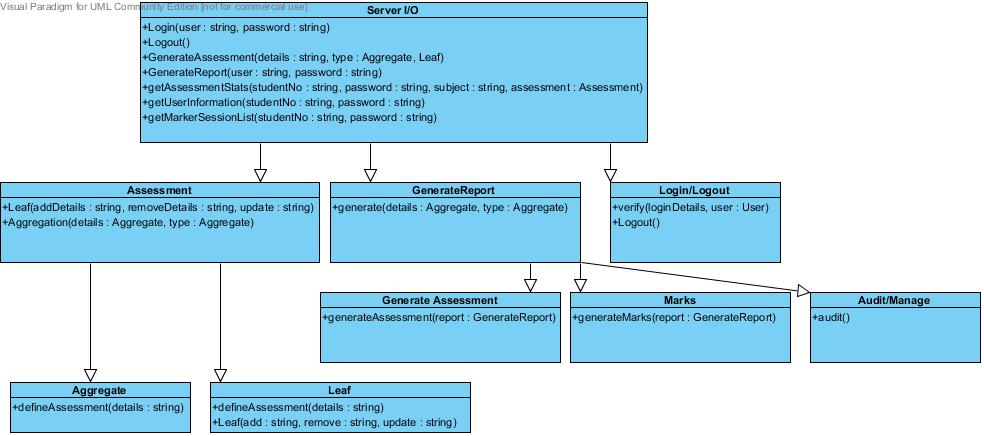
\includegraphics[scale=0.5]{./subdocs/Z/ClassDiagram1.jpg}}
\caption{Class Diagram}
\end{figure}

\subsubsection{System Class diagram}

\begin{figure}[H]
\centering	
\framebox{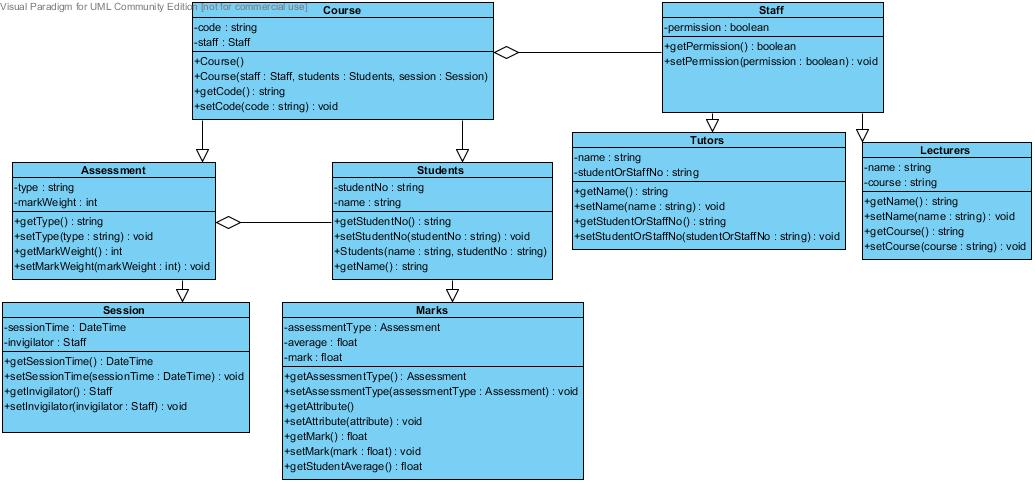
\includegraphics[scale=0.48]{./subdocs/Z/SystemClassDiagram.jpg}}
\caption{System Class diagram}
\end{figure}

\subsubsection{Work-flow}

\begin{figure}[H]
\centering	
\framebox{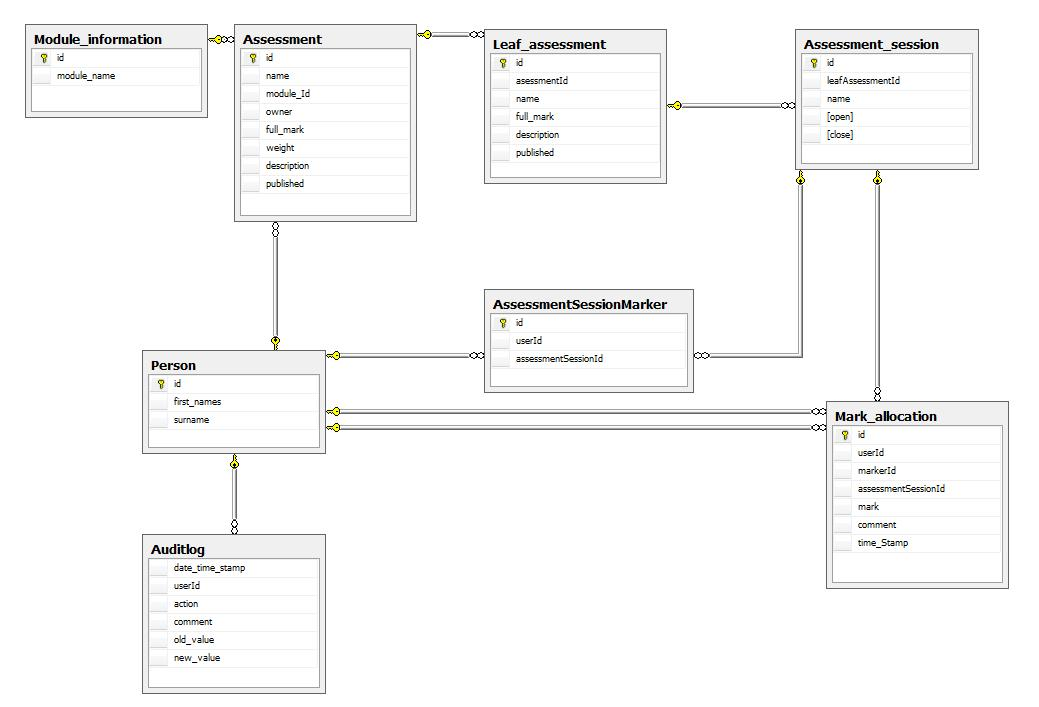
\includegraphics[scale=0.5]{./subdocs/Database/Database.jpg}}
\caption{Activity diagram for user work-flow specifications}
\end{figure}

\subsubsection{Database tables}

\begin{figure}[H]
\centering	
\framebox{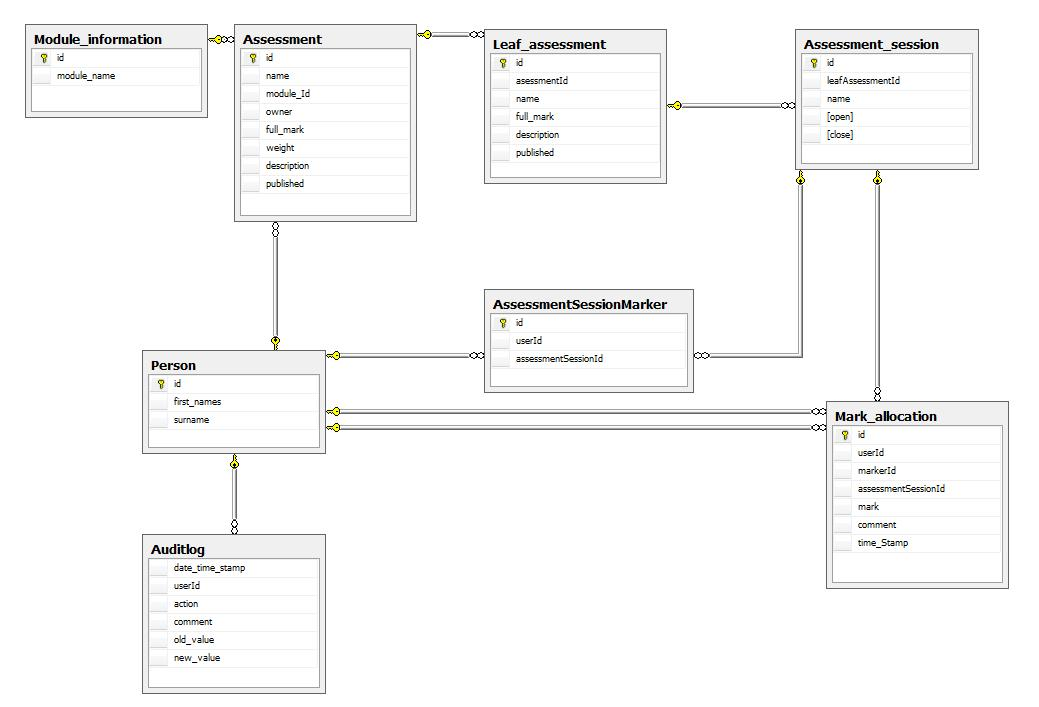
\includegraphics[scale=0.75]{./subdocs/Database/DatabaseDiagram.jpg}}
\caption{Database Diagram}
\end{figure}

%Module information table
\begin{table}[ht]
\begin{tabular}[c]{|p{3cm}||p{2.1cm}||p{1.2cm}||p{1.5cm}||p{2cm}|p{4cm}|}
  \hline
  \multicolumn{6}{|c|}{Module\_Information} \\
  \hline 
  Field & Type & Null & Key & Default & Extra \\ [0.5ex] % Table Heading
  \hline
  id & int(11) & No & Pri & NULL & auto\_increment \\
  name & varchar(255) & No & & & \\
  \hline
\end{tabular}
\end{table} 

%Person table
\begin{table}[ht]
\begin{tabular}[c]{|p{3cm}||p{2.1cm}||p{1.2cm}||p{1.5cm}||p{2cm}|p{4cm}|}
  \hline
  \multicolumn{6}{|c|}{Person} \\
  \hline 
  Field & Type & Null & Key & Default & Extra \\ [0.5ex] % Table Heading
  \hline
  id & int(8) & No & Pri & NULL & auto\_increment \\
  first\_names & varchar(255) & Yes & & NULL & \\
  surname & varchar(255) & No & & & \\
  \hline
\end{tabular}
\end{table} 

Person table:
This table will store only the details of a user that will be used for searching because it is a fast reference, as these and other details about a user is already stored in the LDAP system.

%Auditlog table
\begin{table}[ht]
\begin{tabular}[c]{|p{3cm}||p{2.1cm}||p{1.2cm}||p{1.5cm}||p{2cm}|p{4cm}|}
  \hline
  \multicolumn{6}{|c|}{Auditlog} \\
  \hline 
  Field & Type & Null & Key & Default & Extra \\ [0.5ex] % Table Heading
  \hline
  date\_time\_stamp & datetime & No & & 0000\_00\_00 00:00:00 & \\
  id & int(8) & No & Foreign & & References Person \\
  action & varchar(20) & No & & & See reference 1 \\
  description & varchar(100) & Yes & & NULL & \\
  old\_value & varchar(100) & Yes & & NULL & \\
  new\_value & varchar(100) & No & & & \\
  \hline
\end{tabular}
\end{table} 

Reference 1: Action may have one of the following values: Assessment Created, Assessment Modified, Assessment Removed, Mark Submitted, Mark Modified, Mark Removed, Open Assessment, Close Assessment, Publish Marks, Assessment Report, Students Marks Report, Audit Report.
Auditlog table:
This table will store all changes made to the database except for a mark entered for the first time. The old value can be any type of value for example a session closing datetime which is changed or a mark which is updated, the new value will specify the value which it was changed to.

%Assessment table
\begin{table}[ht]
\begin{tabular}[c]{|p{3cm}||p{2.1cm}||p{1.2cm}||p{1.5cm}||p{2cm}|p{4cm}|}
  \hline
  \multicolumn{6}{|c|}{Assessment} \\
  \hline 
  Field & Type & Null & Key & Default & Extra \\ [0.5ex] % Table Heading
  \hline
  id & int(8) & No & Pri & NULL & auto\_increment \\
  name & varchar(100) & No & & & \\
  module\_id & int(8) & No & Foreign & & References Module\_information \\
  owner & int(8) & No & Foreign & & References Person \\
  weight & int(3) & Yes & & 100 & \\
  best\_of & int(5) & Yes & & 99999 & \\
  description & varchar(255) & Yes & & NULL & \\
  published & bit & No & & False & \\
  \hline
\end{tabular}
\end{table} 

%Leaf_assessment table
\begin{table}[ht]
\begin{tabular}[c]{|p{3cm}||p{2.1cm}||p{1.2cm}||p{1.5cm}||p{2cm}|p{4cm}|}
  \hline
  \multicolumn{6}{|c|}{Leaf\_assessment} \\
  \hline 
  Field & Type & Null & Key & Default & Extra \\ [0.5ex] % Table Heading
  \hline
  id & int(8) & No & Pri & NULL & auto\_increment \\
  name & varchar(100) & No & & & \\
  assessment\_id & int(8) & No & Foreign & & References Assessment \\
  full\_mark & int(3) & No & & & \\
  description & varchar(255) & Yes & NULL & & \\
  published & bit & No & & False & \\
  \hline
\end{tabular}
\end{table} 

Assessment and Leaf\_assessment table:
For example Practical, Tutorial, Semester Test or Exam will be assessments, leaf assessments will be for example Practical 1, Practical 2, Tutorial 1, Tutorial 2, Semester Test 1, Semester Test 2.

%Assessment_session table
\begin{table}[ht]
\begin{tabular}[c]{|p{3cm}||p{2.1cm}||p{1.2cm}||p{1.5cm}||p{2cm}|p{4cm}|}
  \hline
  \multicolumn{6}{|c|}{Assessment\_session} \\
  \hline 
  Field & Type & Null & Key & Default & Extra \\ [0.5ex] % Table Heading
  \hline
  id & int(8) & No & Pri & NULL & auto\_increment \\
  leaf\_assessment\_id & int(8) & No & Foreign & & References Leaf\_assessment \\
  name & varchar(100) & No & & & \\
  open & datetime & No & & Date/time now & \\
  close & datetime & No & & Date/time now & \\
  \hline
\end{tabular}
\end{table} 

Assessment\_session table:
This table will contain all the information needed per session of an assessment.

%Assessment_Session_Marker table
\begin{table}[ht]
\begin{tabular}[c]{|p{3cm}||p{2.1cm}||p{1.2cm}||p{1.5cm}||p{2cm}|p{4cm}|}
  \hline
  \multicolumn{6}{|c|}{Assessment\_Session\_Marker} \\
  \hline 
  Field & Type & Null & Key & Default & Extra \\ [0.5ex] % Table Heading
  \hline
  id & int(8) & No & Pri & NULL & auto\_increment \\
  user\_id & int(8) & No & Foreign & & References Person\\
  assessment\_session\_id & int(8) & No & Foreign & & References Assessment\_session \\
  \hline
\end{tabular}
\end{table} 

Assessment\_Session\_Marker table:
This table will specify which marker is associated with which assessment session.

%Mark_allocation table
\begin{table}[ht]
\begin{tabular}[c]{|p{3cm}||p{2.1cm}||p{1.2cm}||p{1.5cm}||p{2cm}|p{4cm}|}
  \hline
  \multicolumn{6}{|c|}{Mark\_allocation} \\
  \hline 
  Field & Type & Null & Key & Default & Extra \\ [0.5ex] % Table Heading
  \hline
  id & int(8) & No & Pri & NULL & auto\_increment \\
  user\_id & int(8) & No & Foreign & & References Person\\
  marker\_id & int(8) & No & Foreign & & References Person\\
  assessment\_session\_id & int(8) & No & Foreign & & References Assessment\_session \\
  mark & int(3) & No & & & \\
  comment & varchar(255) & Yes & & & \\
  time\_stamp & datetime & No & & & \\
  \hline
\end{tabular}
\end{table} 

Mark\_allocation table:
This table will store all the marks obtained per student per assessment session marked.


